% Auto-generated by analysis/corridor_estimator/run.py --corridor14 -- do not hand-edit.
% Requires \usepackage{subcaption} and \usepackage{graphicx}. Paths are relative to PAPER/ICLR/.
\begin{figure}[t]
  \centering
  \begin{minipage}[c]{0.66\linewidth}
    \centering
    \subcaptionbox{true, exit\label{fig:k40-exit-true}}[0.32\linewidth]{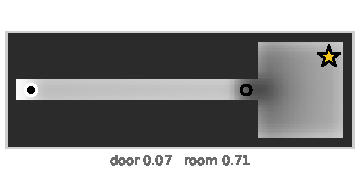
\includegraphics[width=\linewidth]{figures/corridor/k40/exit_true.pdf}}\hfill
    \subcaptionbox{FB, exit\label{fig:k40-exit-fb}}[0.32\linewidth]{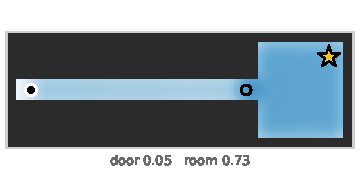
\includegraphics[width=\linewidth]{figures/corridor/k40/exit_fb.pdf}}\hfill
    \subcaptionbox{Density-FB, exit\label{fig:k40-exit-density}}[0.32\linewidth]{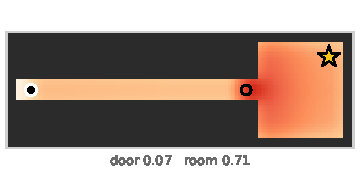
\includegraphics[width=\linewidth]{figures/corridor/k40/exit_density.pdf}}\\[0.4em]
    \subcaptionbox{true, fail\label{fig:k40-fail-true}}[0.32\linewidth]{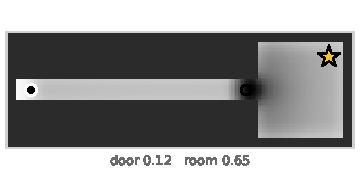
\includegraphics[width=\linewidth]{figures/corridor/k40/fail_true.pdf}}\hfill
    \subcaptionbox{FB, fail\label{fig:k40-fail-fb}}[0.32\linewidth]{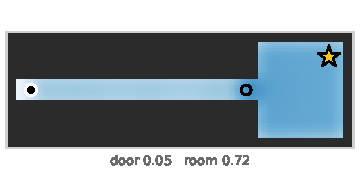
\includegraphics[width=\linewidth]{figures/corridor/k40/fail_fb.pdf}}\hfill
    \subcaptionbox{Density-FB, fail\label{fig:k40-fail-density}}[0.32\linewidth]{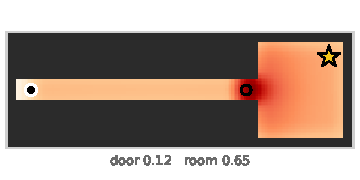
\includegraphics[width=\linewidth]{figures/corridor/k40/fail_density.pdf}}\\[0.4em]
    \subcaptionbox{true, fail $-$ exit\label{fig:k40-contrast-true}}[0.32\linewidth]{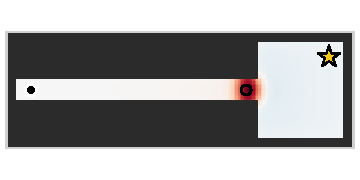
\includegraphics[width=\linewidth]{figures/corridor/k40/contrast_true.pdf}}\hfill
    \subcaptionbox{FB, fail $-$ exit\label{fig:k40-contrast-fb}}[0.32\linewidth]{
\includegraphics[width=\linewidth]{figures/corridor/k40/contrast_fb.pdf}}\hfill
    \subcaptionbox{Density-FB, fail $-$ exit\label{fig:k40-contrast-density}}[0.32\linewidth]{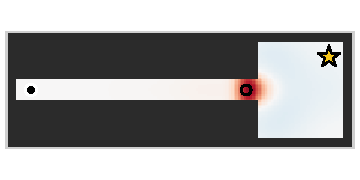
\includegraphics[width=\linewidth]{figures/corridor/k40/contrast_density.pdf}}\\[0.3em]
    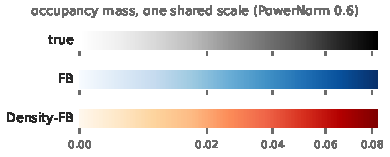
\includegraphics[width=0.42\linewidth]{figures/corridor/k40/colorbar_occ.pdf}\hfill
    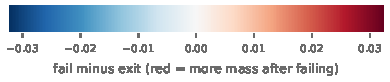
\includegraphics[width=0.42\linewidth]{figures/corridor/k40/colorbar_contrast.pdf}
  \end{minipage}\hfill
  \begin{minipage}[c]{0.32\linewidth}
    \centering
    \subcaptionbox{margin at $D$ vs.\ $k$\label{fig:k40-margin}}[\linewidth]{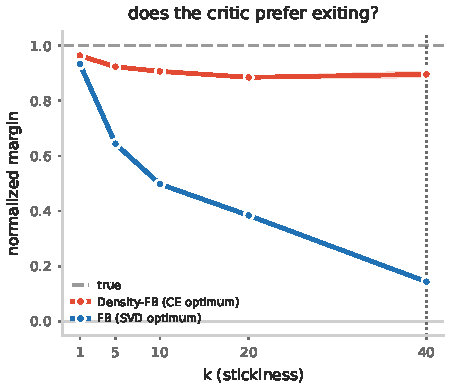
\includegraphics[width=\linewidth]{figures/corridor/k40/margin_vs_k.pdf}}
  \end{minipage}
  \caption{Corridor with exit, 14 corridor cells, agent starting at the first corridor cell (black dot; hollow marker = exit $D$, star = far room cell), at stickiness $k{=}40$, rank $d{=}8$, $\gamma{=}0.98$, closed-form fits (FB: rank-$d$ SVD optimum of its $\rho$-weighted squared loss; Density-FB: rank-$d$ softmax cross-entropy optimum, seed 0).
    Rows: occupancy after walking to $D$ and exiting (a--c), after walking to $D$ and taking a failing action (d--f), and the signed difference fail minus exit (g--i; red = more mass after failing).
    Occupancy maps share one PowerNorm(0.6) scale (left colorbar; hue = estimator); contrast maps share one symmetric scale fixed to the true contrast's largest entry (right colorbar).
    The number line under each map is the mass fraction on $D$ and inside the room.
    $|\Delta|/|\Delta_{\mathrm{true}}|$: FB 0.23, Density-FB 1.02; TV of the contrast map to the true contrast: FB 0.05, Density-FB 0.02.
    Right: normalized value margin at $D$ (exit minus mean failing action, divided by the true margin) versus $k$; dotted line = the $k$ shown on the left.}
  \label{fig:corridor-k40}
\end{figure}
